\documentclass[14pt, a4paper]{extarticle}

\usepackage{graphicx}
\graphicspath{{./images/}}
\DeclareGraphicsExtensions{.jpg,.png}
\usepackage{csvsimple}

\usepackage{amsfonts}
\usepackage{amsmath}

\usepackage[english,russian]{babel}

\usepackage{fontspec} 
\defaultfontfeatures{Ligatures={TeX},Renderer=Basic}
\setmainfont[Ligatures={TeX,Historic}]{Times New Roman}
\setmonofont{Courier New}
\newfontfamily\cyrillicfonttt[Script=Cyrillic]{Courier New}

\usepackage{xcolor}

\usepackage{tabularx}

\usepackage{indentfirst} %отступ первой строки первого абзаца
\linespread{1.25}

\usepackage{geometry}
\geometry{left=3cm}
\geometry{right=1cm}
\geometry{top=2cm}
\geometry{bottom=2cm}

\setlength{\parindent}{1.25cm}

\usepackage{enumitem}
\setlist{left=\parindent, labelsep=1cm, itemsep=0pt, topsep=0pt}

\usepackage[final]{pdfpages}

\usepackage{titlesec} % оформление заголовков

\titleformat{\section}[block]
	{\newpage\hspace{\parindent}\bfseries\fontsize{18pt}{21.6pt}\selectfont}
        {\thesection}
        {1em}{\MakeUppercase}
\titleformat{name=\section,numberless}[block]
	{\newpage\centering\bfseries\fontsize{18pt}{21.6pt}\selectfont}
        {}
        {1em}{}
\titleformat{\subsection}[block]
	{\bfseries\hspace{\parindent}\fontsize{16pt}{19.2pt}\selectfont}
        {\thesubsection}
        {1em}{}

\usepackage{etoolbox}

\usepackage{nameref}
\usepackage{hyperref}
\hypersetup{
    colorlinks,
    citecolor=black,
    filecolor=black,
    linkcolor=black,
    urlcolor=black
}
\urlstyle{same}
        
\usepackage{float}
\usepackage{caption}

\usepackage{newfloat}
\DeclareCaptionType[name=Листинг, placement=htbp]{listing}

\usepackage{fancyvrb}

\DeclareCaptionLabelSeparator{emdash}{\;\textemdash\;}
\captionsetup[figure]{name={Рисунок}, labelsep=emdash, justification=centering, position=above, singlelinecheck=off, font={small, bf}, labelfont=bf, skip=6pt}
\captionsetup[table]{name={Таблица}, labelsep=emdash, justification=raggedright, position=top, singlelinecheck=off, font={small, it}, labelfont=it, skip=6pt}
\captionsetup[listing]{name={Листинг}, labelsep=emdash, justification=raggedright, position=top, singlelinecheck=off, font={small, it}, labelfont=it, skip=-16pt}

\counterwithin{figure}{section}
\counterwithin{table}{section}
\counterwithin{listing}{section}

\usepackage{array}
\newcommand\ChangeRT[1]{\noalign{\hrule height #1}}

\usepackage{ragged2e}
\usepackage{microtype}

\justifying
\sloppy
\tolerance=500
\hyphenpenalty=10000
\emergencystretch=3em

\usepackage{setspace}

\usepackage{multirow}

\usepackage[
citestyle=gost-numeric,
style=gost-numeric, 
backend=biber
]{biblatex}
\addbibresource{prac.bib}
\usepackage{calc}
\defbibenvironment{bibliography}
  {\list{\printfield[labelnumberwidth]{labelnumber}}
    {\setlength{\leftmargin}{0pt}%
     \setlength{\itemindent}{\parindent}%
     \setlength{\labelsep}{1.5em}%
     \addtolength{\itemindent}{\labelsep+\labelnumberwidth}%
     \setlength{\itemsep}{\bibitemsep}%
     \setlength{\parsep}{\bibparsep}}}
  {\endlist}
  {\item}
\DeclareFieldFormat{urldate}{(Дата обращения: #1)}

\begin{document}

\makeatletter
\renewcommand{\l@section}{\@dottedtocline{1}{0em}{1.25em}}
\renewcommand{\l@subsection}{\@dottedtocline{2}{0em}{1.75em}}
\renewcommand{\l@subsubsection}{\@dottedtocline{3}{0em}{2.6em}}
\renewcommand{\@dotsep}{1.25}
\makeatother

\def\contentsname{СОДЕРЖАНИЕ}

\pagenumbering{gobble}
\begin{titlepage}

\includepdf{title}
\end{titlepage}
\tableofcontents

\section*{ВВЕДЕНИЕ}
\pagenumbering{arabic}
\setcounter{page}{3}
\addcontentsline{toc}{section}{ВВЕДЕНИЕ}

Это пример документа на \LaTeX, в котором представлены все элементы, необходимые для отчётов/курсача/практической.

\section{ТАБЛИЦЫ}

\subsection{Пример на tabularx}
tabularx позволяет задавать ширину таблицы (например по ширине страницы).\cite{overleaf-tables}

Пример оформления таблицы:
\begin{table}[H]
\caption{Таблица истинности для данной функции}
\small
\centering
\label{tab1}
\begin{tabular}{!{\vrule width 1.75pt} c | c | c | c | c !{\vrule width 1.75pt} c !{\vrule width 1.75pt}}
\ChangeRT{1.75pt}
$x_1$ & $x_2$ & $x_3$ & $x_4$ & $x_5$ & $x_6$ \\ \ChangeRT{1.75pt}
0 & 0 & 0 & 0 & 0 & 0 \\ \hline
0 & 0 & 0 & 0 & 1 & 0 \\ \hline
0 & 0 & 0 & 1 & 0 & 0 \\ \hline
0 & 0 & 0 & 1 & 1 & 1 \\ \hline

0 & 0 & 1 & 0 & 0 & 0 \\ \hline
0 & 0 & 1 & 0 & 1 & 0 \\ \hline
0 & 0 & 1 & 1 & 0 & 1 \\ \hline
0 & 0 & 1 & 1 & 1 & 1 \\ \hline

0 & 1 & 0 & 0 & 0 & 0 \\ \hline
0 & 1 & 0 & 0 & 1 & 0 \\ \hline
0 & 1 & 0 & 1 & 0 & 1 \\ \hline
0 & 1 & 0 & 1 & 1 & 1 \\ \hline

0 & 1 & 1 & 0 & 0 & 0 \\ \hline
0 & 1 & 1 & 0 & 1 & 0 \\ \hline
0 & 1 & 1 & 1 & 0 & 1 \\ \hline
0 & 1 & 1 & 1 & 1 & 1 \\ \hline

1 & 0 & 0 & 0 & 0 & 1 \\ \hline
1 & 0 & 0 & 0 & 1 & 0 \\ \hline
1 & 0 & 0 & 1 & 0 & 0 \\ \hline
1 & 0 & 0 & 1 & 1 & 1 \\ \hline

1 & 0 & 1 & 0 & 0 & 1 \\ \hline
1 & 0 & 1 & 0 & 1 & 1 \\ \hline
1 & 0 & 1 & 1 & 0 & 0 \\ \hline
1 & 0 & 1 & 1 & 1 & 0 \\ \hline

1 & 1 & 0 & 0 & 0 & 1 \\ \hline
1 & 1 & 0 & 0 & 1 & 1 \\ \hline
1 & 1 & 0 & 1 & 0 & 0 \\ \hline
1 & 1 & 0 & 1 & 1 & 0 \\ \hline

1 & 1 & 1 & 0 & 0 & 1 \\ \hline
1 & 1 & 1 & 0 & 1 & 1 \\ \hline
1 & 1 & 1 & 1 & 0 & 1 \\ \hline
1 & 1 & 1 & 1 & 1 & 1 \\ \ChangeRT{1.75pt}
\end{tabular}
\end{table}

``ChangeRT'' --- заранее заданная фукнция, которая изменяет толщину горизонтальной линии.
\subsection{Пример на tabular}

\begin{table}[H]
\centering
\small
\caption{Импликантная таблица}
\label{tab:impl}
\begin{tabular}{!{\vrule width 1.75pt} c | c !{\vrule width 1.75pt} c | c | c | c | c | c | c | c | c !{\vrule width 1.75pt}}
\ChangeRT{1.75pt}
         &       & $S_1$   & $S_2$ & $S_3$   & $S_4$ & $S_5$ & $S_6$ & $S_7$ & $S_8$ & $S_{9}$  \\ \hline
         &       & 1-{}-00 & -0011 & 0-{}-11 & 0-11- & 01-1- & 1-10- & 11-0- & -111- & 111-{}- \\ \hline
         &       &         &       &         &       &       &       &       &       &         \\ \ChangeRT{1.75pt}
$P_1$    & 00011 &         & 1     & 1       &       &       &       &       &       &         \\ \hline
$P_2$    & 00110 &         &       &         & 1     &       &       &       &       &         \\ \hline
$P_3$    & 00111 &         &       & 1       & 1     &       &       &       &       &         \\ \hline
$P_4$    & 01010 &         &       &         &       & 1     &       &       &       &         \\ \hline
$P_5$    & 01011 &         &       & 1       &       & 1     &       &       & 1     &         \\ \hline
$P_6$    & 01110 &         &       &         & 1     & 1     &       &       &       &         \\ \hline
$P_7$    & 01111 &         &       & 1       & 1     & 1     &       &       & 1     &         \\ \hline
$P_8$    & 10000 & 1       &       &         &       &       &       &       &       &         \\ \hline
$P_9$    & 10011 &         & 1     &         &       &       &       &       &       &         \\ \hline
$P_{10}$ & 10100 & 1       &       &         &       &       & 1     &       &       &         \\ \hline
$P_{11}$ & 10101 &         &       &         &       &       & 1     &       &       &         \\ \hline
$P_{12}$ & 11000 & 1       &       &         &       &       &       & 1     &       &         \\ \hline
$P_{13}$ & 11001 &         &       &         &       &       &       & 1     &       &         \\ \hline
$P_{14}$ & 11100 & 1       &       &         &       &       & 1     & 1     &       & 1       \\ \hline
$P_{15}$ & 11101 &         &       &         &       &       & 1     & 1     &       & 1       \\ \hline
$P_{16}$ & 11110 &         &       &         &       &       &       &       & 1     & 1       \\ \hline
$P_{17}$ & 11111 &         &       &         &       &       &       &       & 1     & 1       \\ \ChangeRT{1.75pt}
\end{tabular}
\end{table}

\section{ФОРМУЛЫ}

\ref{func:mdnf-karno} --- однострочная формула
\ref{func:patrick} --- многострочная формула

\begin{equation}\centering\label{func:mdnf-karno}
F_\text{МДНФ}=x_1x_2\bar{x_3} \vee x_1x_3\bar{x_4} \vee x_1\bar{x_4}\bar{x_5} \vee \bar{x_1}x_2x_4 \vee \bar{x_1}x_3x_4 \vee \bar{x_2}\bar{x_3}x_4x_5 \vee x_1x_2x_3
\end{equation}

\begin{center}
\onehalfspacing
\vspace{-2em}
\begin{align}
1 = (S_{2} \vee S_{3}) \wedge S_{4} \wedge (S_{3} \vee S_{4}) \wedge S_{5} \wedge (S_{3} \vee S_{5} \vee S_{8}) \wedge (S_{4} \vee S_{5}) \wedge (S_3 \vee S_4 \vee S_5 \vee \nonumber
\end{align}
\vspace{-4em}
\begin{align}
\vee S_8) \wedge S_1 \wedge S_2 \wedge (S_1 \vee S_6) \wedge S_6 \wedge (S_1 \vee S_7) \wedge S_7 \wedge (S_1 \vee S_6 \vee S_7 \vee S_9) \wedge (S_6 \vee \nonumber
\end{align}
\vspace{-4em}
\begin{align}
\vee S_7 \vee S_9) \wedge (S_8 \vee S_9) \wedge (S_8 \vee S_9) \nonumber
\end{align}
\end{center}
\begin{center}
\onehalfspacing
\vspace{-2em}
\begin{align}
1 = S_1S_2S_4S_5S_6S_7S_8 \vee S_1S_2S_4S_5S_6S_7S_9 \vee S_1S_2S_3S_4S_5S_6S_7S_8 \vee \nonumber
\end{align}
\vspace{-4em}
\begin{align}
 \vee S_1S_2S_3S_4S_5S_6S_7S_9 \vee S_1S_2S_4S_5S_6S_7S_8S_9 \vee S_1S_2S_3S_4S_5S_6S_7S_8S_9. \label{func:patrick}
\end{align}
\end{center}

\section{РИСУНКИ}

Пример картинки (Рисунок\;\ref{fig:bukh1}), bukh\_1 --- название .png файла. 

\begin{figure}[H]
\centering
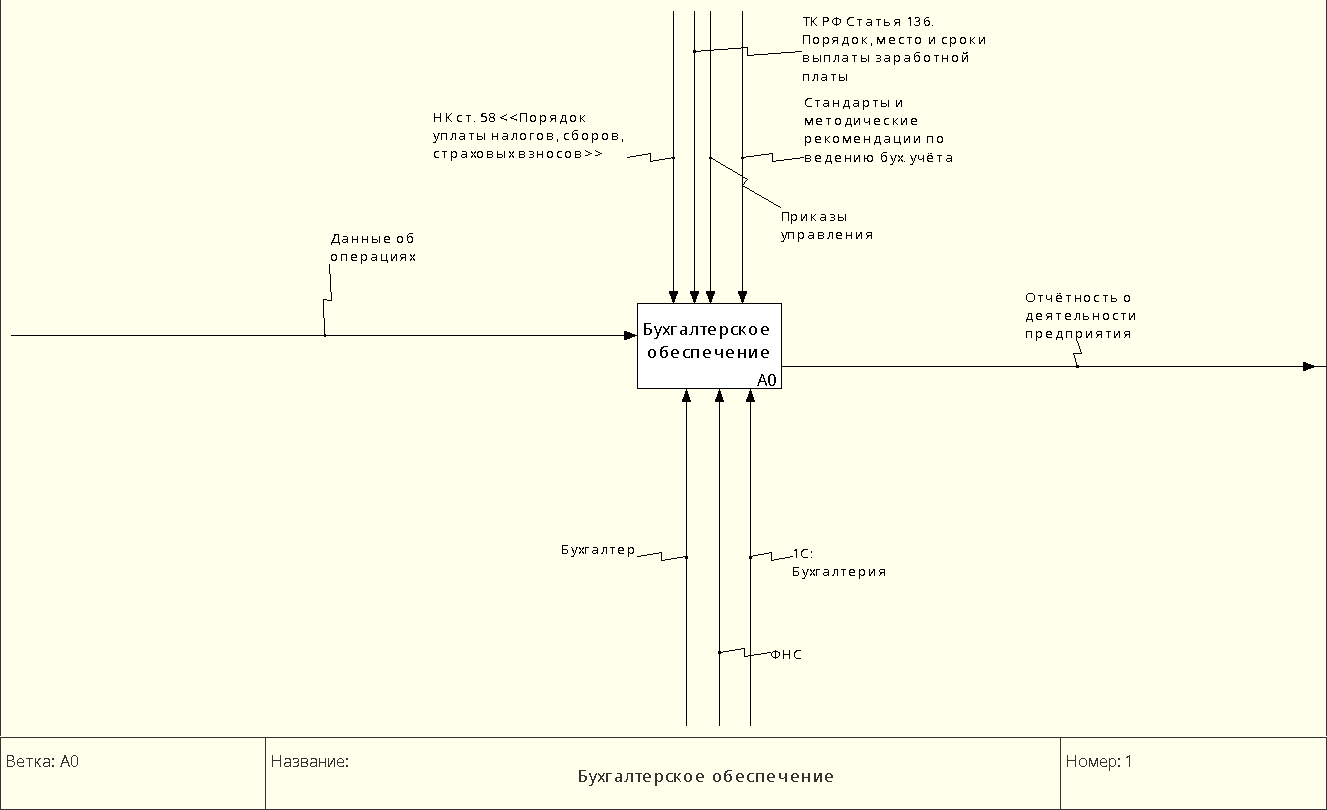
\includegraphics[scale=0.45]{bukh_1}
\caption{Первый уровень процесса бухгалтерского обеспечения\label{fig:bukh1}}
\end{figure}

\section{ЛИСТИНГИ}

Пример листинга представлен ниже.

\begin{listing}[H]
\caption{Реализация автомата\label{list:fsm}}
\begin{Verbatim}[frame=single, fontsize=\footnotesize]
`timescale 1ns / 1ps

module fsm(
        input m, n, clk, 
        output reg [3:0] state,
        output reg [15:0] out
    );
\end{Verbatim}
\end{listing}
\begin{listing}[H]
\caption*{Продолжение листинга\;\ref{list:fsm}}
\begin{Verbatim}[frame=single, fontsize=\footnotesize]
    initial
    begin
        state <= 0;
        out <= 16'd4563;
    end
    always @(posedge clk)
    begin
        case(state)
            4'd0: begin
                state <= 4'd1;
                out <= 16'd1432;
            end
            4'd1: begin
                if(m) begin
                    state <= 4'd3;
                    out <= 16'd695;
                end else begin
                    state <= 4'd2;
                    out <= 16'd7;
                end
            end
            4'd2: begin
                if(m) begin
                    state <= 4'd4;
                    out <= 16'd9912;
                end else begin
                    if(n) begin
                        state <= 4'd5;
                        out <= 16'd6554;
                    end else begin
                        state <= 4'd2;
                        out <= 16'd7;
                    end
                end
             end
             4'd3: begin
                if(m) begin
                    if(n) begin
                        state <= 4'd5;
                        out <= 16'd6554;
                    end else begin
                        state <= 4'd6;
                        out <= 16'd7056;
                    end
                end else begin
                        state <= 4'd3;
                        out <= 16'd695;
                end
             end
             4'd4: begin
                if(m) begin
                    state <= 4'd5;
                    out <= 16'd6554;
                end else begin
                    state <= 4'd4;
                    out <= 16'd9912;
                end
             end
\end{Verbatim}
\end{listing}

\section*{ЗАКЛЮЧЕНИЕ} 
\addcontentsline{toc}{section}{ЗАКЛЮЧЕНИЕ}
Я показал примеры оформления различных элемнтов отчёта. Всё что вам нужно сделать это написать текст и использовать данные примеры для своих отчётов. Писать в \textbf{XeLaTeX}\cite{overleaf-xelatex} можно при помощи онлайн редактора Overleaf\cite{overleaf}.

Список используемых источников редактируется в файле ``prac.bib''.

Титульный лист --- title.pdf. Редактируется в функции includepdf{title}
\printbibliography[title=СПИСОК ИСПОЛЬЗУЕМЫХ ИСТОЧНИКОВ]\addcontentsline{toc}{section}{СПИСОК ИСПОЛЬЗУЕМЫХ ИСТОЧНИКОВ}
\end{document}